\documentclass[
    ngerman,american
    ]{scrartcl}

    % ##########################################
    % # Choose the language for the document by editing below line
    % # de = German
    % # en = English
    \newcommand{\lang}{en}
    % ##########################################

    \usepackage{babel}
    \usepackage[pdftex]{graphicx,color}
    \usepackage[utf8]{inputenc} 
    \usepackage{csquotes}
    \usepackage{enumitem}
    \usepackage{ifthen}
    \usepackage{lipsum}
    
    \newcommand{\paperSubTitle}[1]
{
    \ifthenelse{\equal{#1}{en}}{Outline and Topic Proposal}{}
    \ifthenelse{\equal{#1}{de}}{Outline und Themenvorschlag}{}
}

\newcommand{\sectionQuestions}[1]
{
    \ifthenelse{\equal{#1}{en}}{\section{Scope of Work - 4 Questions}}{}
    \ifthenelse{\equal{#1}{de}}{\section{Ziel der Arbeit - 4 Fragen}}{}
}

\newcommand{\sectionQuestionsDescription}[1]
{
    \ifthenelse{\equal{#1}{en}}{In this section the essence of the proposed work is described by answering four key questions. }{}
    \ifthenelse{\equal{#1}{de}}{Im Folgenden wird der Kern der Arbeit beschrieben indem vier Kernfragen beantwortet werden.}{}
}

\newcommand{\sectionInitialTOC}[1]
{
    \ifthenelse{\equal{#1}{en}}{\section{Preliminary Table of Contents}}{}
    \ifthenelse{\equal{#1}{de}}{\section{Vorläufige Gliederung}}{}
}

\newcommand{\sectionInitialTOCDescription}[1]
{
    \ifthenelse{\equal{#1}{en}}{In this section the table of contents for the proposed work is described.}{}
    \ifthenelse{\equal{#1}{de}}{Im Folgenden wird ein Inhaltverzeichnis für die vorgeschlagene Arbeit vorgestellt.}{}
}

\newcommand{\sectionSource}[1]
{
    \ifthenelse{\equal{#1}{en}}{\section{Relevant Related Work}}{}
    \ifthenelse{\equal{#1}{de}}{\section{Relevante verwandte Arbeiten}}{}
}


\newcommand{\sectionSourceDescription}[1]
{
    \ifthenelse{\equal{#1}{en}}{In this section, identified related work is described.}{}
    \ifthenelse{\equal{#1}{de}}{Diese Section stellt verwandte Arbeiten dar und erklärt kurz deren Bedeutung für die vorgeschlagene Arbeit.}{}
}

\newcommand{\questionOne}[1]
{
    \ifthenelse{\equal{#1}{en}}{What is the problem you want to address in your work?}{}
    \ifthenelse{\equal{#1}{de}}{Was ist das Problem, welches Sie in Ihrer Arbeit bearbeiten wollen?}{}
}

\newcommand{\questionTwo}[1]
{
    \ifthenelse{\equal{#1}{en}}{Why is it a problem?}{}
    \ifthenelse{\equal{#1}{de}}{Warum ist es ein Problem?}{}
}

\newcommand{\questionThree}[1]
{
    \ifthenelse{\equal{#1}{en}}{What is the solution you developed in your work?}{}
    \ifthenelse{\equal{#1}{de}}{Was ist die Lösung die sie entwickelt haben?}{}
}

\newcommand{\questionFour}[1]
{
    \ifthenelse{\equal{#1}{en}}{Why is it a solution?}{}
    \ifthenelse{\equal{#1}{de}}{Warum ist es eine Lösung?}{}
}


    \ifthenelse{\equal{en}{\lang}}
    {
        \selectlanguage{american} 
    }{
        \ifthenelse{\equal{de}{\lang}}
        {
            \selectlanguage{ngerman}
        }
        {\selectlanguage{american}}        
    }
 
    \usepackage[
        bibencoding=utf8, 
        style=alphabetic
    ]{biblatex}

    \bibliography{bibliography}
    
    
    \usepackage{amsmath}
    \title{
        % ##########################################
        % # Insert the title of your paper/thesis here
        % ###### 
        % Coming up with a good title is hard.
        % It should:
        %  1. capture the contents of the your work
        %  2. not be to broad or generic
        %  3. stick to the truth and don't not oversell
        %  4. use established terms and wordings
        %  5. make people curious about your work
        %  6. use current buzzwords if possilbe (but do it right)
        %  7. not use too many buzzwords :-)
        ApakoHa - an automated tool 
        \\ using dynamic taint analysis
        \\ for android security focusing on sensitive data
        % ##########################################
        \\  \Large{\paperSubTitle{\lang}}} % don't touch this line

    \author{
        % ##########################################
        % # Your name goes here
        % ######
        % wWll, that should be obvious, right? 
        Kaiyuan Xu, Yiwei Yang, Zhe Ye, Longwen Zhang
        % ##########################################
        }
    
    \begin{document}
      \maketitle
        \begin{abstract}

            \ifthenelse{\equal{en}{\lang}}{}{}
            % ##########################################
            % # Include your Abstract here 
            % ######
            % I would strongly suggest to start working on the abstract only 
            % after you have answered the 4 questions in Section 1, as this will
            % make it much easier for you to come up with an abstract that
            % is to the point, short, and still summarizing all the most crucial 
            % results of your work.
            %
            % The abstract should include the following points:
            %  - a short but to the point introduction of the problem area
            %  - what is the topic/problem, tackled in your work? 
            %  - why is the topic/problem of your work relevant? Why should the 
            %    reader care about it?
            %  - what are the results/answers of your work?
            %  - how did you gain your results and what is their quality?
            %                %  
            % It should NOT be:
            %  - too long/verbose
            %  - too short
            Android security has attracted much research attention from both academy 
            and industry recently. Dynamic Taint Analysis(DTA) is a classic analysis to detect
             information flow problems and it has been widely adopted to detect private
             data leaks in Android applications. In this project, we will automate the
             process of taint analysis and provide more detailed information about the dataflow on both the source code 
             and the byte-code. Thus providing a way for Maple IR to continue to compile.
             % ##########################################

        \end{abstract}
        
        
        \sectionQuestions{\lang}
        \sectionQuestionsDescription{\lang}
        
        \begin{description}[style=unboxed]
            \item [\questionOne{\lang}] 
                % ##########################################
                % # Question 1: What is the problem you want to address in your work? / 
                %               Was ist das Problem, welches Sie in Ihrer Arbeit bearbeiten wollen?
                % ######
                % The goal of this question is to clearly state what your work is about. 
                % What is the problem it is supposed to solve?
                %
                % Answering this question is particular important during the early phases 
                % of your work, in order to gain further insight and understanding about what 
                % your work is going to cover and address.  
                %
                % Answer this question very briefly by stating the problem or research 
                % question that you want to address/solve in your work.
                % 
                % Your answer should: 
                %  - only be 1 sentence (2 sentences max)
                %  - not cover a statement why the topic is relevant 
                %    for the industry (this is address by the next question)
                %  - properly use common terms and buzzwords of IT today (similar to the 
                %    rules for the abstract)
                %
                % Please acknowledge: the answer to this question should not cover why the 
                % problem/Users/victoryang00/Documents/rCore/crate/memory/src/ is important or relevant to anyone (e.g. industry). This will 
                % be addressed with the next question.
                People can't perform the DTA on their apps on the ART runtime fast. Nowadays, DTA consumes time to set up environments and may receive invalid results.  
                % ##########################################

            \item [\questionTwo{\lang}]
                % ##########################################
                % # Question 2: Why is it a problem? / Warum ist es ein Problem?
                % ######
                % The goal of this question is to describe why your work is relevant. 
                % Why should the reader care? Why is this the problem (of question 1)
                % worth investigating?
                %
                % Answering this question is particular important during the early phases 
                % of your work, in order to gain further insight and understanding of the 
                % problem domain you are addressing. Further, it is a good checkpoint to 
                % ensure that you are addressing issues that are not just theoretical but 
                % have real-world applications. 
                %
                % Your answer should: 
                %  - be 3 - 5 sentences 
                %  - give a broader overview of the domain/area where your problem occurs
                %  -- who has this problem?
                %  -- what is the impact of it?
                %  -- which conditions need to be fulfilled for the problem to occur?
                %  -- etc.
                %  - describe the benefit of having the problem resolved
                Generally, researchers detect privacy leaks and analyze related data flows. One is static analysis, that is, decompiling a given app, and performing static stain analysis or symbolic execution on the obtained code. , Such as FlowDroid, the advantage is that it can widely obtain the trend of private data, but it does not include runtime information. When app developers use technologies such as java reflection mechanism or code encryption, static analysis basically cannot handle this, and The overhead is large, and it takes tens of times more time of compiling time to complete. The second is dynamic analysis, modifying the system or system library, or instrumenting the app, so that the app at runtime can be monitored. An important task of using dynamic stain analysis technology to detect the information flow of the Android system is TaintDroid. However, TaintDroid is based on the Dalvik virtual machine for taint propagation, and currently only supports Android 4.3 at the highest.
                % ##########################################

            \item [\questionThree{\lang}]
                % ##########################################
                % # Question 3: What is the solution you developed in your work? / 
                %               Was ist die L?sung die sie entwickelt haben?
                % ######
                % The goal of this question is to describe the results of your work 
                % ans/or solution to the problem of your work.
                % 
                % It is hard/impossible to answer this question in the early phases of 
                % your work, as usually you do not have results, yet. However, you can 
                % already state first ideas that you may have in order to discuss them 
                % with your supervisor. 
                %
                % Your answer should:
                %  - clearly state all results of your work, that are relevant to your 
                %    research problem. 
                %  - not oversell your results, stick you what you actually have 
                %    accomplished"
                %  - give credit where credit is due. If you created your results based 
                %    on the work of others, give them the credit.
                %  - if none of your ideas did not produce any usable solution, state 
                %    so - these attempts are also results! By documenting them, it may 
                %    prevent others from trying them as well. 
                We proposed to adapt the TaintART to automated DTA tools that we demands. \\
                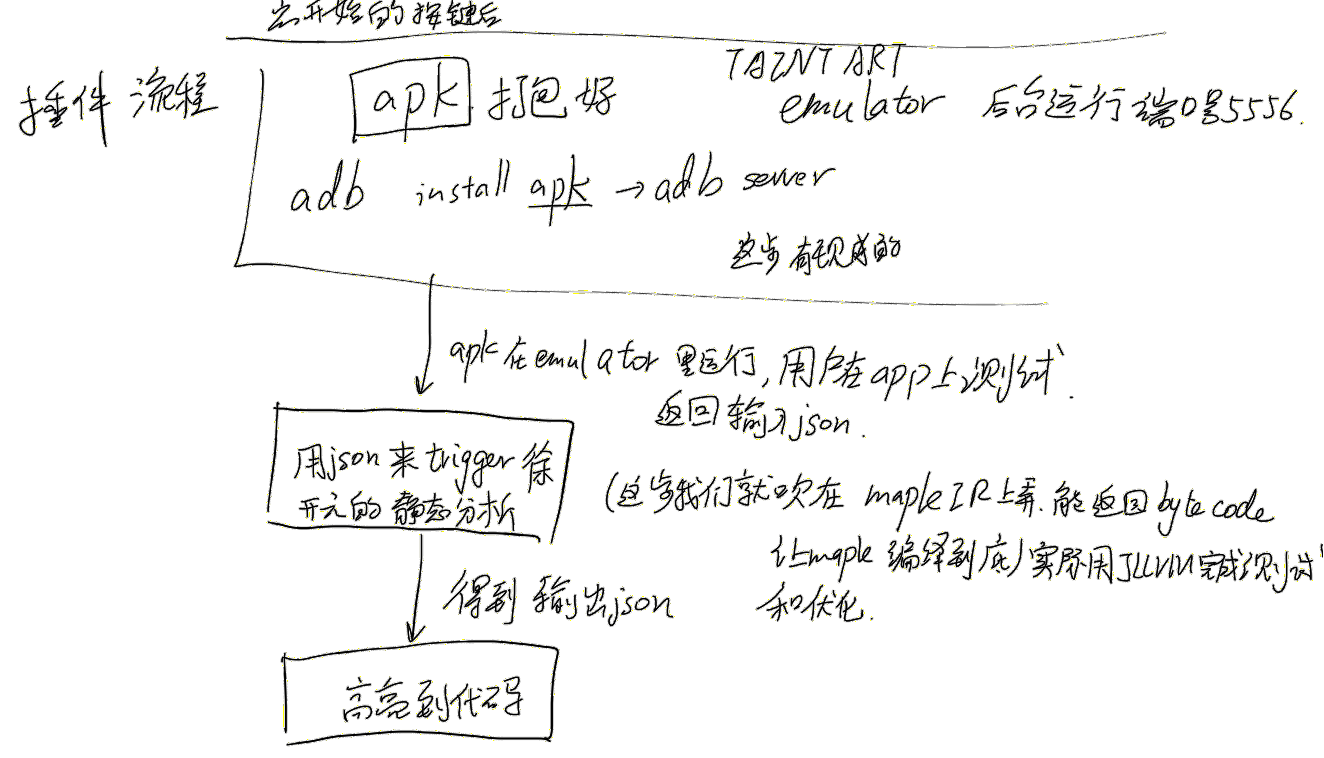
\includegraphics[width=10cm]{1.png}\\
                The source code is transferred to the qemu x86 64 virtual machine. Coverted to ART Runtime executable by dex2oat
                implemented with llvm. In this step, TaintART performs a spot instrumentation operation. At runtime, TaintART uses the general-purpose register R5 to store the tags of the variables in the register, R1 to 3 passes the parameters between the methods, and R12 cooperates with the transfer of the internal operation of the register. A specific area is opened on the heap to store the stain information, so that the stain propagation logic can be detected To information leakage or potentially malicious behavior. After returning to the host, it will use JLLVM Pass (this step can be replaced with Maple IR phase) to perform static control flow analysis on the stain information and corresponding functions and APIs, and finally return it to the developer. The developer can modify the source code or use Pass to improve development efficiency. The final bytecode will enable Maple IR to generate the target.\\
                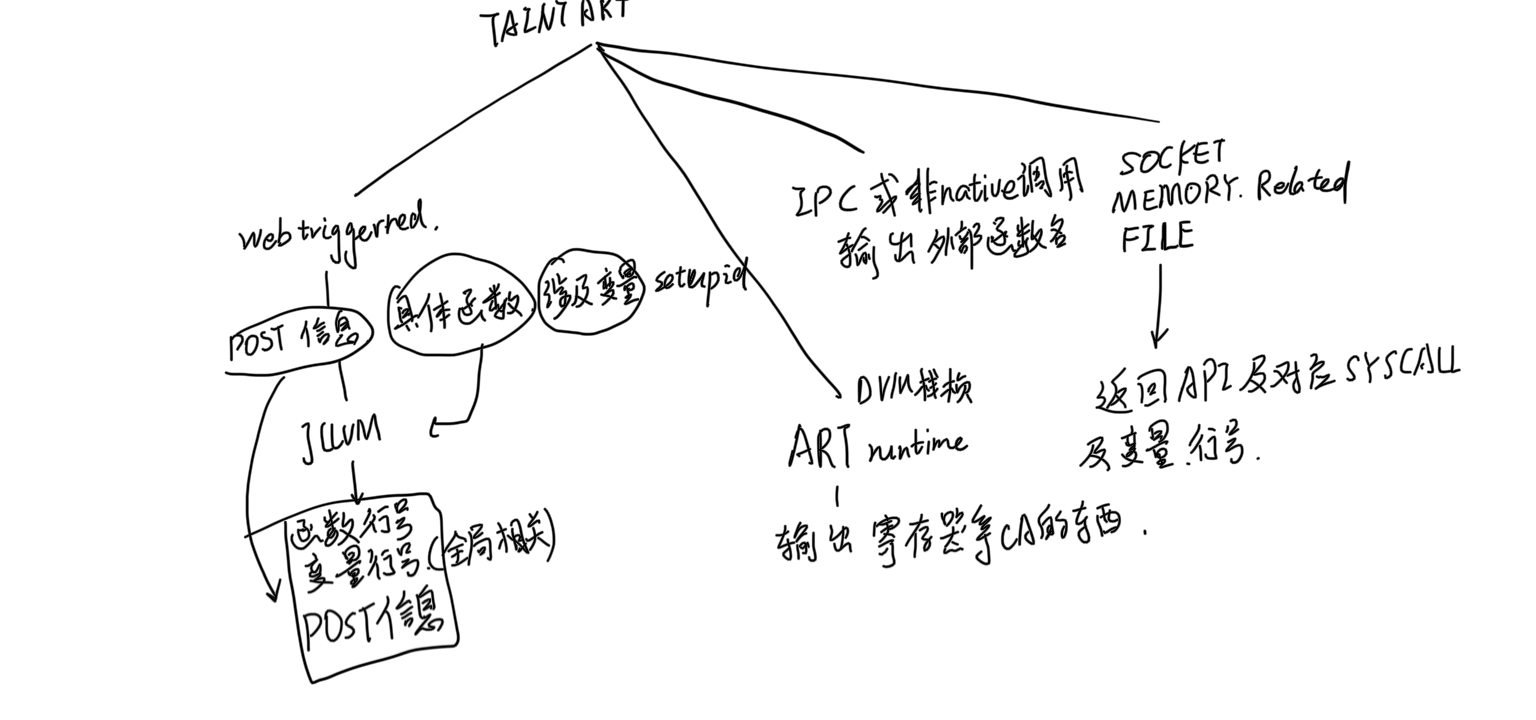
\includegraphics[width=10cm]{2.png}\\
                As for the information of different source(like web, IPC, socket or memory and files), we adopt different methods to deal with.
                % ##########################################

            \item [\questionFour{\lang}]
                % ##########################################
                % # Question 4: Why is it a solution? / Warum ist es eine L?sung?
                % ######
                % The goal of this question is to describe who you developed your results 
                % and what the quality of them are.
                % 
                % Your answer should:
                %  - short and to the point
                %  - clearly state how you developed your results
                %  -- what is the chain of reasoning that led to your results/solution
                %  -- what statistics, literature, studies, or other literature did you 
                %     base your assumptions on?
                %  - clearly state the quality and applicability of your results
                %  -- reflect your work objectively - there is no perfection in this 
                %     world, so your work is not perfect as well. Be aware of that!
                %  -- how did you ensure that your results are accurate? did you:
                %  --- perform experiments? 
                %  --- apply any logical deductions?
                %  --- mathematical proofs? 
                %  --- implement a "proof of concept" implementation and evaluate? 
                %  --- etc.
                %  - clearly state the shortcomings of your work
                %  -- be hones and objective about your own work. 
                %  -- In which cases/scenarios are your results applicable?
                The reason we use x86 64 virtual machine is to raise the speed in case of cross ISA compilation. The reason to use static analysis is to get a more precise information of the control flow graph which is the shortage of DTA.
                We will apply the benchmark and a demo to show that our solution is faster and more focused privacy.
                % ##########################################
        \end{description}
        
        \sectionInitialTOC{\lang}
        \sectionInitialTOCDescription{\lang}
        
        % ##########################################
        % # Proposed table of contents
        % ######
        % The goal of this section is to propose a table of contents. Please keep in
        % mind: a well created table of contents is very powerful in provide a good 
        % overview of the overall chain of reasoning of your work. This makes it 
        % extremely valuable.
        % 
        % Please include:
        %  - names of sections and subsections (please don't go deeper than that unless 
        %    your supervisor asks you for it)
        %  - a brief description of the proposed content of each section and subsection
        %    (1-3 sentences)
        % 
        \begin{enumerate}
            \item \textbf{Introduction} How android information privacy security evolves
                    \begin{enumerate}
                        \item \textbf{from DVM to ART} 
                        \item \textbf{from STA to DTA} 
                    \end{enumerate}
            \item \textbf{The basics of ApakoHa principle} How The steps go
                    \begin{enumerate}
                        \item \textbf{how DTA is realized in TaintART} 
                        \item \textbf{how to second-develop TaintART}
                        \item \textbf{JLLVM pass}
                        \item \textbf{the combination of STA and DTA} 
                    \end{enumerate}
            \item \textbf{Case Study} How our tools preform in real test.
                    \begin{enumerate}
                        \item \textbf{simplified TouTiao}
                        \begin{enumerate}
                            \item \textbf{Benchmark compared with state of art of android privacy detection tools} comparisan with a JIT-based java STA
                            \item \textbf{Benchmark with TaintDroid} Will TaintART get the bugs as TaintDroid do
                            \item \textbf{The app developers feedback} will the developer use the plugin 
                        \end{enumerate}
                    \end{enumerate}
            \item \textbf{Division of Duty} insert brief description
                    \begin{enumerate}
                        \item \textbf{Kaiyuan XU} implement the JLLVM pass.
                        \item \textbf{Zhe YE} implement the VScode plugin
                        \item \textbf{Longwen ZHNAG} second-develop TaintART
                        \item \textbf{Yiwei YANG} Propose the Idea and do TainART realization
                        % \item \textbf{Subsection 2 Name} insert brief description
                    \end{enumerate}
        \end{enumerate}
        % ##########################################
    
      
        \sectionSource{\lang}
        \sectionSourceDescription{\lang}

        % ##########################################
        % # Overview of identified relevant work
        % ######
        % The goal of this section is to provide an overview of the relevant and significant 
        % related work identified so far. Make sure that your cited sources are of appropriate
        % quality!
        % 
        % Please include:
        %  - a citation of the source using Latex facilities (incl. a generated list of 
        %    references)
        %  - a brief descriptions of the source and a statement why this is relevant for 
        %    your work (1-2 sentences)
        % 
        \begin{description}
        \item[\cite{Sun:2016:TPM:2976749.2978343}] A Practical Multi-level Information-Flow Tracking System for Android RunTime
        \item[\cite{WCNCW.2019.8902627}] Android Malware Detection Based on System Calls Analysis and CNN Classification
        \item[\cite{SPW.2018.00031}] A Dynamic Taint Analysis Tool for Android App Forensics
        \item[\cite{NGMAST.2014.23}] Android Malware Detection Using Parallel Machine Learning Classifiers
        \item[\cite{IMIS.2014.28}] PasDroid: Real-Time Security Enhancement for Android
        \end{description}
        % ##########################################
        
        
    \end{document}